\documentclass{beamer}
\usetheme[navigation]{UMONS}
\usepackage[utf8]{inputenc}
\usepackage[frenchb]{babel}
\usepackage{graphicx}
\newcommand{\tabitem}{~~\llap{\textbullet}~~}
\newcommand{\incinslide}[1]{
\begin{figure}
 \centering
 \includegraphics[height=6.5cm]{../figures/#1}
\end{figure}}

% title page informations
\title[Projet de Master 1]{Un réseau de neurones pour la\\
\includegraphics[height=1cm]{../sphero.jpg}}
\author[J. Bury]{Jason Bury}
\institute[]{
 Faculté des Sciences\\
  Université de Mons
  \\[2ex]
  
\includegraphics[height=4ex]{../UMONS.jpg}\hspace{2em}%
  \raisebox{-1ex}{
\includegraphics[height=6ex]{../FS_Logo.jpg}}
}

\begin{document}
\maketitle

\section{Sphero}
\subsection{Qu'est ce?}

\begin{frame}
 \frametitle{Présentation de la Sphero}
\end{frame}

\subsection{Design du vecteur d'entrée}
\subsubsection{Données utiles}
Avant de choisir le réseau de neurones à utiliser pour Générer des commandes pour la Sphero, il est important d'identifier ce que nous souhaitons obtenir en sortie et les informations que nous pouvons fournir en entrée en omettant les données inutiles.
Si le vecteur d'entrée est de dimension très grande, alors un réseau \rbf devra avoir un trop grand nombre de neurones cachés\cite{Gauthier}.
Si nous supposons que la sortie produite peut dépendre non seulement de l'input actuel mais aussi des entrées précédentes, alors un réseau récurrent devra être utilisé.

La Sphero peut nous fournir:\cite{SDKofficiels}
\begin{itemize}
 \item Sa position grâce à un odomètre (cm),
 \item Son vecteur vitesse (mm/s),
 \item Son vecteur d'accélération grâce à un accéleromètre (mG),
 \item Son orientation (-179$\rightarrow$180 degrés),
 \item Son niveau de charge (Pas de poucentage mais label \enum{Chargement}, \enum{OK}, \enum{Bas} et \enum{Critique}),
 \item État des LEDs, évènement de collision, voltage de la batterie, nombre de charges, version ...
\end{itemize}

Parmis ces données, nous n'avons pas besoin de l'état des LEDs, version et nombre de charges car ils n'influencent pas la conduite de la Shero.
Dans ce projet, nous ne prenons pas en compte les éventuels collisions.

Le niveau de charge pourrait influencer la conduite.
Nous ne savons pas si la puissance maximale des moteurs diminuent lorsque la charge est trop faible.
Si cela s'avère être le cas, pour ne pas devoir effectuer un entrainement pour chaque niveau de charge différent, on entrainera la Sphero que pour les cas où le niveau de charge est à \enum{OK} et on supposera donc que la conduite sera effectuée qu'avec ce niveau de charge.

Un odomètre n'est pas approprié pour la mesure de position dans notre application.
En effet, la distance parcourue n'est mesurée qu'à partir du roulement du moteur permettant le déplacement.
La distance parcourue par dérapage ne sera pas comptabilisée.
Cela a été vérifié lors de l'expérience menée dans la section \ref{sec:choixdesign}.
Une camera sera utilisée pour tracer la position réelle de la Sphero.

Pour l'accélération, les commandes à appliquer à l'instant $t$ ne dépendent pas de l'accélération à l'instant $t$ juste avant l'application des commandes.
Mais par contre, cette donnée peut être utile pour anticiper la vitesse de la Sphero au moment où elle reçoit les commandes car du à la latence d'envoi de paquet, la vitesse à l'instant $t$ n'est plus la même que celle communiquée.
Si cette donnée impacte peu dans les résultats obtenus, alors nous pourrions décider de nous passer de ce paramètre.
Ajouter cette dimension dans le vecteur d'entrée demandera un plus grand nombre d'exemples pour la phases d'apprentissage car il faut balayer toutes les configurations possibles de vecteur d'entrée.

\newcommand{\inchist}[1]{
 \begin{minipage}{0.48\textwidth}
  \includegraphics[width=10cm]{../figures/hist#1.jpeg}
 \end{minipage}
}
\subsubsection{Choix du design}\label{sec:choixdesign}
 %TODO montrer les design repris chez gauthier
Pour une meilleure précision, on ajoute un vecteur vitesse à atteindre sur le point de destination.
On aligne l'axe des abscisses avec l'axe de l'orientation du moteur afin de reduire le domaine d'entrée et donc le nombre d'exemples à créer pour l'apprentissage.
Le vecteur d'entrée contiendra donc le vecteur vitesse, la position relative à atteindre dans $T$ secondes où $T$ sera la période à laquelle on échantillonera les données des capteurs.
Nous avons donc un vecteur d'entrée à 6 dimensions (vitesse actuelle en x et y, position relative cible en x et y, vitesse cible en x et y).
Le vecteur de sortie sera la puissance à donner pour chaque moteur.

Estimons la valeur optimale que nous pouvons donner à $T$.
Une commande de streaming de donnée peut être envoyée à la Sphero.
Grâce à cette commande, nous pouvons demander à la Sphero d'envoyer uniquement les données qui nous interessent à une fréquence donnée.
Trois paramètres de cette commande peuvent influencer les performances d'échantillonage:
\begin{enumerate}
 \item Un diviseur (entier) de la fréquence maximale d'échantillonage.
 \item Le nombre d'échantillonage à garder en mémoire avant envoi.
 \item Le nombre de capteur à échantilloner.
\end{enumerate}
Un échantillonage consiste à obtenir seulement les données qui nous intéressent à un instant précis.
La fréquence maximale d'échantillonage, un échantillon à la fois, est de 400Hz.\cite{SDKofficiels}
La vitesse maximale de la Sphero est de 4,5 miles par heure.\cite{product} Ce qui fait environ 2 mètres par seconde.
\begin{figure}
 \centering
 \inchist{20}
 \inchist{40}
 \inchist{60}
 \inchist{80}
 \inchist{100}
 \inchist{200}
 \caption{Histogrammes de temps de réception de packet streamé. Générés via script R}
 \label{histogrammes}
\end{figure}

À la Figure \ref{histogrammes} sont repris les histogrammes de temps de réceptions de paquets pour différentes fréquences d'échantillonage.
En plus du streaming, pour chaque paquet reçu, un paquet est envoyé à la Sphero pour changer les leds.
Cela nous permet d'obtenir des résultats qui se rapprocheront de ce que nous obtiendrons si nous envoyons une nouvelle commande à chaque période $T$.
La configuration de l'ordinateur utilisé est la suivante:
\begin{itemize}
 \item AMD Athlon(tm) X2 Dual-Core QL-64
 \item Carte mère EI Capitan
 \item 3 Go de RAM DDR2
 \item disque dur ST9250827AS 5400rpm
 \item Adapteur USB bluetooth BT009x, transfert 1Mbs.
 \item OS: Linux 4.4.0-57-generic, Ubuntu 16.04.4
\end{itemize}

On observe tout d'abord que les temps de réception ont l'air de suivre une cadence de 1ms.
Cela peut s'expliquer par le fait que la Sphero 2.0 a une granularité de 1ms pour l'éxecution de macro.\cite{product}
%Plus $T$ est petit, plus notre système de commande est réactif et, toutes choses égales par ailleur, nous pouvons effectuer des mouvements plus précis.
Pour les critères de choix d'une valeur pour $T$, deux critères sont pris en compte:
\begin{enumerate}
 \item La stabilité du streaming. Moins la densité de probabilité de temps de réception de paquet est concentrée sur le voisinage de $T$, moins la solutions sera précise.
 \item Le temps de réaction. Plus $T$ est grand, moins la trajectoire de la Sphero sera fidèle à la trajectoire voulue.
 Nous pouvons compenser ce manque de précision par un vecteur d'entrée plus complexe mais la solution converge alors moins vite et un ensemble d'apprentissage plus conséquent doit être fournis.
\end{enumerate}

On observe que la stabilité du streaming varie selon la fréquence.
Prenons le streaming à 60Hz. On observe que en moyenne les paquets arrivent toutes les 15 millisecondes.
La distance maximale que peut parcourir la Sphero en 15ms est de 3 cm.
Le manque de précision dû au temps de réaction est dans ce cas négligeable pour des trajectoires à grande vitesse de l'ordre de quelque mètres.
De plus, ce streaming étant le plus stable, c'est cette fréquence qui sera utilisée.
Nous considèrerons donc que $T$ = 15ms malgré que la fréquence est règlée à 60Hz.


\section{Les NN}

\begin{frame}
 \frametitle{Sélection d'un réseau de neurones}
 
\end{frame}

\subsection{Perceptron multi-couches}
\begin{frame}
 \frametitle{Perceptron multi-couches}
 \framesubtitle{Un neurone}
 
\end{frame}

\begin{frame}
 \frametitle{Perceptron multi-couches}
 \framesubtitle{Fonctions d'activation}
 
\end{frame}

\begin{frame}
 \frametitle{Perceptron multi-couches}
 \framesubtitle{Les couches}
 
\end{frame}

\subsection{Fonction à base radiale}
\begin{frame}
 \frametitle{Fonction à base radiale}
 \framesubtitle{Un neurone}
 
\end{frame}

\begin{frame}
 \frametitle{Fonction à base radiale}
 \framesubtitle{Les couches}
 
\end{frame}

\subsection{Réseau de neurones récursif}
\begin{frame}
  \frametitle{Perceptron multi-couches récurrent}
  \framesubtitle{Un neurone}
  
\end{frame}

\begin{frame}
  \frametitle{Perceptron multi-couches récurrent}
  \framesubtitle{Les couches}
  
\end{frame}

\section{Méthodes d'apprentissage avec maître distant}
Nous allons observer différentes architectures intéressantes dans le cas de génération de commandes.
Le mot \enum{architecture} utilisé ici ne désigne pas l'architecture d'un réseau de neurones mais l'architecture d'une méthode d'utilisation de réseaux de neurones.
La convention graphique est montré dans la Figure \ref{legendearchi}.
\begin{figure}
 \centering
 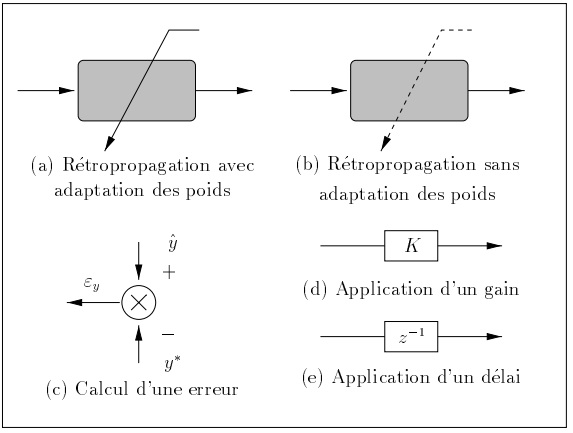
\includegraphics[scale=0.6]{../figures/applegende.jpg}
 \caption{Conventions graphiques pour la descriptions de l'architecture d'une méthode utilisant des RNA. \textbf{Source}: Gauthier\cite{Gauthier}}
 \label{legendearchi}
\end{figure}

\subsection{Le problème}
Dans cette section, nous allons voir différentes méthodes pour entrainer un réseau de neurones à générer des commandes.
Ces méthodes visent à contourner le \emph{problème de l'apprentissage avec maître distant}.
Dans l'apprentissage supervisé, un \emph{maître} est ce qui permet de fournir une erreur entre la sortie d'un réseau de neurones et la sortie attendue.
Et effectivement dans notre cas, nous n'avons rien qui puisse nous permettre de définir les commandes idéales à éxécuter pour passer d'un certain état à l'autre.
Par contre nous pouvons avoir un maître qui compare l'état résultant de l'exécution d'une commande à l'état cible.

Dans les figures qui suivront, Système désigne l'exécution, dans la réalité, de la commande entrée.
En sortie du Système nous avons l'état résultat de l'exécution des commandes.

\subsection{Reproduction d'un contrôleur}
\begin{figure}
 \centering
 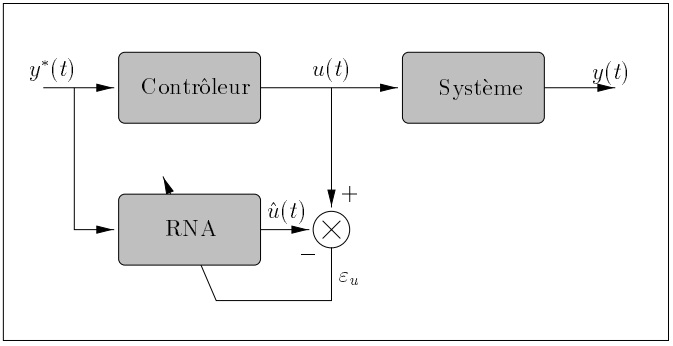
\includegraphics[scale=0.5]{../figures/appsimple.jpg}
 \caption{Apprentissage par reproduction d'un contrôleur. \textbf{Source}: Gauthier\cite{Gauthier}}
 \label{appcontroleur}
\end{figure}
Dans cette méthode d'apprentissage, le \rna apprend à reproduire les commandes d'un contrôleur existant (\textbf{Figure \ref{appcontroleur}}).
Cette méthode a été utilisé pour commander le volant d'une voiture pour suivre des virages où le controlleur est un humain.\cite{Pomerleau}

\subsection{Apprentissage spécialisé}\label{sec:appspecial}
\begin{figure}
 \centering
 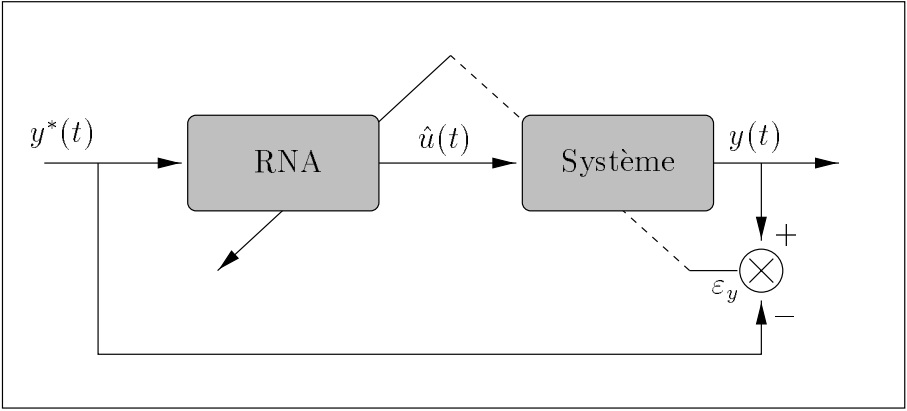
\includegraphics[scale=0.4]{../figures/appspecialise.jpg}
 \caption{Apprentissage spécialisé. \textbf{Source}: Gauthier\cite{Gauthier}}
 \label{appspecialise}
\end{figure}
Ici on applique l'algorithme de rétropropagation en démarrant depuis le maître distant et en passant par le système.
Par exemple, nous avons vu que, dans le cas d'un \mlp, section \ref{sec:appmlp}, l'apprentissage est l'application de la formule \[\Delta W_{ij} = -\eta\partiel{Q}{W_{ij}} = \partiel{Q}{\phi_i} \partiel{\phi_i}{v_i} \partiel{v_i}{W_{ij}}\]
En reprenant la notation de la Figure \ref{appspecialise}, \[\Delta W_{ij} = -\eta\partiel{\varepsilon_y}{W_{ij}} = \partiel{\varepsilon_y}{\hat{u}} \partiel{\hat{u}}{v_i} \partiel{v_i}{W_{ij}}\]
Où $v_i$ est la somme pondérée des entrées du neurones $i$.
Or $\partiel{\varepsilon_y}{\hat{u}} = \partiel{\varepsilon_y}{y}\partiel{y}{\hat{u}}$. Et donc la formule devient
\[\Delta W_{ij} = \partiel{\varepsilon_y}{y} \partiel{y}{\hat{u}} \partiel{\hat{u}}{v_i} \partiel{v_i}{W_{ij}}\]
Et définir le facteur $\partiel{y}{\hat{u}}$ est la difficulté de cette méthode:
Il faut pouvoir modèliser le système par une fonction $y(\hat{u})$ dérivable en $\hat{u}$.
%TODO et dans le cas d'un RBF ?

\subsection{Apprentissage en deux phases}\label{sec:app2phases}
\begin{figure}
 \centering
 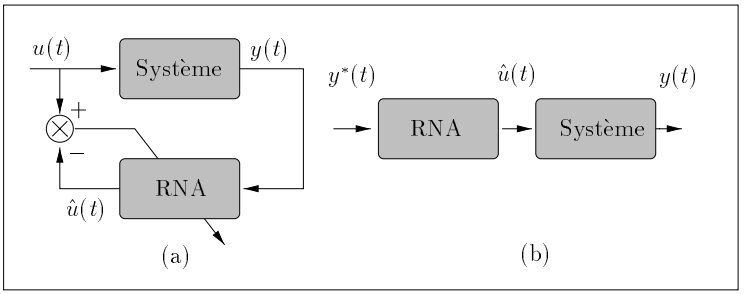
\includegraphics[scale=0.5]{../figures/app2phases.jpg}
 \caption{Apprentissage en deux phases. \textbf{Source}: Gauthier\cite{Gauthier}}
 \label{app2phases}
\end{figure}

Tout d'abord, (a) On génère des commandes $u$ en boucle et on les applique au système (\textbf{Figure \ref{app2phases}}).
Soit $y$ l'état du robot après avoir appliqué la commande $u$, on obtient en boucle des paires entrée/sortie où $y$ est l'entrée et $u$ la cible.
On continue la boucle pour balayer toutes les configurations possibles de $u$.

Puis vient la phase d'utilisation (b) où on utilise le réseau cette fois pour génèrer les commandes. Mais sans apprentissage. L'adaptabilité est donc sacrifiée.\\

Cette méthode est inadapté dans les cas où il existe plusieurs commandes idéales pour un même état cible.
En effet, imaginons qu'il existe deux commandes idéales pour atteindre le même état cible et que ces deux commandes soient rencontrées lors de la phase (a).
Alors les poids seront modifiés pour que la sortie converge vers la première commande idéale rencontrée, puis l'autre et ainsi de suite.
Et finalement, la sortie du réseau pour cet état cible ne va pas converger vers une des commandes idéales.

\subsection{Apprentissage indirecte}\label{sec:appindirect}
\begin{figure}
 \centering
 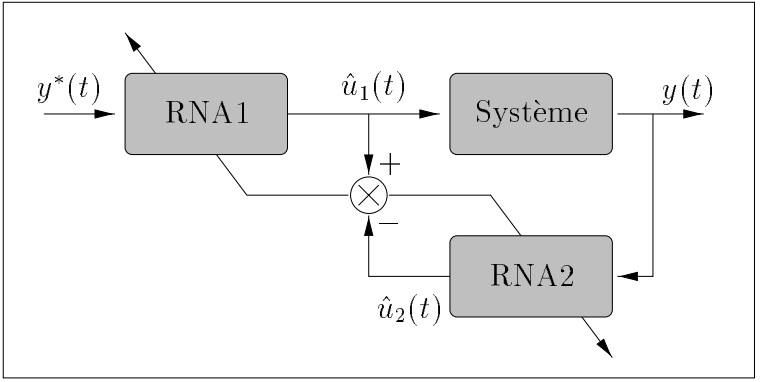
\includegraphics[scale=0.5]{../figures/appindirect.jpg}
 \caption{Apprentissage indirect. \textbf{Source}: Gauthier\cite{Gauthier}}
 \label{appindirect}
\end{figure}
L'apprentissage indirecte, montré dans la \textbf{Figure \ref{appindirect}}, est une méthode qui permet de retrouver l'adaptabilité. (sacrifiée dans l'apprentissage en deux phases, section \ref{app2phases})
RNA1 et RNA2 ne sont pas deux réseaux différents. Il s'agit du même réseau de neurones.
RNA1 et RNA2 partagent les mêmes poids.
Mais selon Gauthier\cite{Gauthier}, cette méthode tend à toujours donner la même commande.

\subsection{Apprentissage par modèle différentiable}\label{sec:appmodele}
\begin{figure}
 \centering
 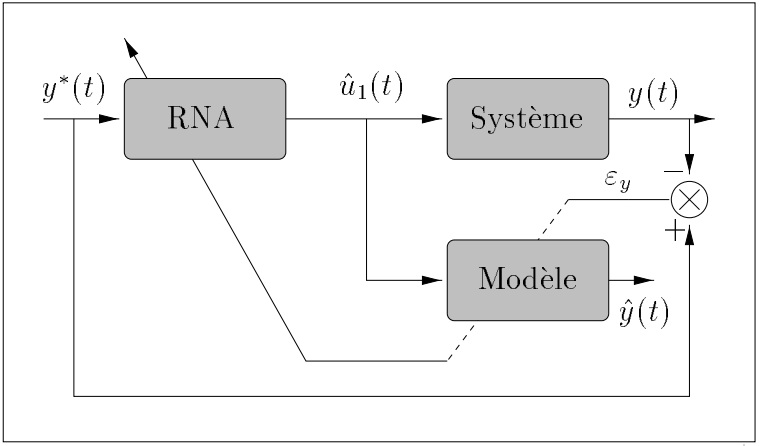
\includegraphics[scale=0.5]{../figures/modelediferentiable.jpg}
 \caption{Apprentissage par modèle différentiable. \textbf{Source}: Gauthier\cite{Gauthier}}
 \label{appmodele}
\end{figure}

L'idée est d'utiliser la méthode de l'apprentissage spécialisé à la section \ref{sec:appspecial} mais en se servant d'un \rna comme modèle différentiable (\textbf{Figure \ref{appindirect}}).
Il faut donc, dans un premier temps, établir un \rna qui va apprendre à prédire le prochain état selon la commande à exécuter.
Nous n'avons pas le problème de l'apprentissage avec maître distant pour ce \rna car sa sortie peut directement être comparée à la sortie du système.
Ensuite, on l'utilise comme modèle. Et là nous pouvons connaître $\partiel{\varepsilon_y}{\hat{u}_1}$ grâce aux formule de rétropropagation de la section \ref{sec:appmlp}.\\
%TODO prouver et parler aussi de formule de backpropagation pour rbf

L'adaptabilité est sacrifiée car si le système change et que le modèle n'a pas été entrainé pour ce nouveau système, l'algorithme de rétropropagation va faire converger la solution vers des commandes inadaptés pour le nouveau système.

\subsection{Apprentissage sur plusieurs étapes}
Un autre problème qui peut se présenter pour la commande par réseaux de neurones est d'obtenir un maître distant seulement après plusieurs étapes.
Par exemple, imaginons que nous voulons commander la marche d'un robot avec un réseau de neurones qui fournira des commandes tous les $T$ secondes.
Si le robot tombe et que nous pouvons en obtenir un maître, nous ne savons pas à quelles étapes avant la chute le réseau a fourni des commandes responsables de cette chute.\\

Une solution à ce problème est l'architecture de Nguyen et Widrow, Figure \ref{appNguyenWidrow}.
\begin{figure}
 \centering
 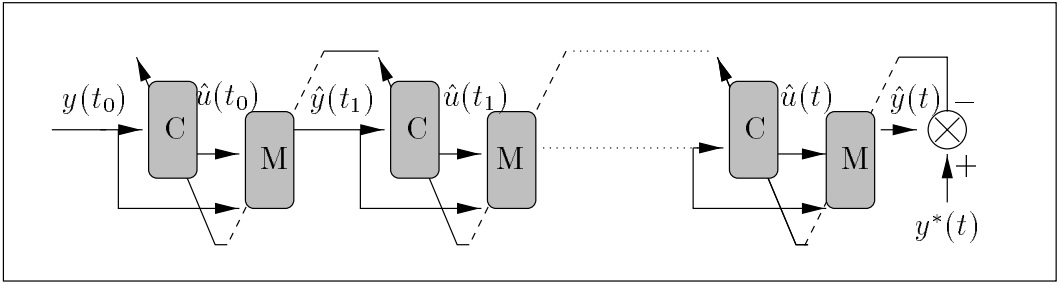
\includegraphics[scale=0.5]{../figures/appNguyenWidrow.jpg}
 \begin{itemize}
  \item \textbf{C}: Réseau qui génère les commandes
  \item \textbf{M}: Modèle
 \end{itemize}
 \caption{Architecture de Nguyen et Widrow. \textbf{Source}: Gauthier\cite{Gauthier}}
 \label{appNguyenWidrow}
\end{figure}
Cela consiste à utiliser un modèle différentiable (qui peut être un réseau de neurone) pour pouvoir effectuer l'algorithme de rétropropagation jusque la première étape après l'obtention du maître précédent.

\section{Implémentation}
\subsection{Implémentation}

\begin{frame}
 \frametitle{Implémentation d'un réseau de neurones feedforward}
 \framesubtitle{Propriété intéressante}
 
\end{frame}

\begin{frame}
 \frametitle{Implémentation d'un réseau de neurones feedforward}
 \framesubtitle{Diagramme de classe}
 
\end{frame}

\begin{frame}
 \frametitle{Implémentation du système de commande}
 \framesubtitle{Modularité}
 
\end{frame}

\begin{frame}
 \frametitle{Implémentation du système de commande}
 \framesubtitle{Diagramme de classe}
 
\end{frame}

\begin{frame}
 \frametitle{Implémentation d'une Sphero virtuelle}

\end{frame}

\section{Commandes aléatoires}
\subsection{Système de commande aléatoire}

\begin{frame}
 \frametitle{Système de commande aléatoire}
 \framesubtitle{Récupération de la trajectoire}
 
\end{frame}

\begin{frame}
 \frametitle{Système de commande aléatoire}
 \framesubtitle{Les problèmes à éviter}
 
\end{frame}


\section{Données}
\subsection{La Sphero virtuelle}

\begin{frame}
 \frametitle{Streaming d'une Sphero virtuelle}
 \framesubtitle{L'orientation}
 
\end{frame}

\begin{frame}
 \frametitle{Streaming d'une Sphero virtuelle}
 \framesubtitle{La vitesse}
 
\end{frame}

\subsection{La Sphero réelle}

\begin{frame}
 \frametitle{Streaming de la Sphero réelle}
 \framesubtitle{L'orientation}
 
\end{frame}

\begin{frame}
 \frametitle{Streaming de la Sphero réelle}
 \framesubtitle{La vitesse}
 
\end{frame}

\section{Résultats des modèles}
\subsection{Pour les 3 réseaux utilisés}

\begin{frame}
 \frametitle{Résultats des modèles générés}
 \framesubtitle{Venant de 3 sources différentes}
 
\end{frame}

\begin{frame}
 \frametitle{Résultats des modèles de Weka}
 \framesubtitle{L'orientation}
 
\end{frame}

\begin{frame}
 \frametitle{Résultats des modèles de Weka}
 \framesubtitle{La vitesse}
 
\end{frame}

\begin{frame}
 \frametitle{1 nearest neighbor}
 \framesubtitle{L'orientation}
 
\end{frame}

\begin{frame}
 \frametitle{1 nearest neighbor}
 \framesubtitle{La vitesse}
 
\end{frame}

\section{Conclusion}
\subsection{Conclusion}
\begin{frame}
 \frametitle{Conclusion}
 
\end{frame}

\end{document}